
%(BEGIN_QUESTION)
% Copyright 2006, Tony R. Kuphaldt, released under the Creative Commons Attribution License (v 1.0)
% This means you may do almost anything with this work of mine, so long as you give me proper credit

Tenk deg frem til funksjonen til alle pressostater og releer i denne kontrollkretsen for en damp generator. Hva betyr diagnostikk meldingene?

$$\includegraphics[width=15.5cm]{i00221x01.eps}$$

Forklar også betydningen av brytersymbolet: NO i forhold til NC. Tidsreleet er spesielt viktigh her. 

\vskip 10pt

Til slutt skal du legge til en bryter for lampetest. Denne skal "teste" alle lamper når en byrter trykkes inn. Finn også ut hvor i NEK EN 60204-1 det settes krav til kampetest for alarmlys. 

\vskip 20pt \vbox{\hrule \hbox{\strut \vrule{} {\bf Suggestions for Socratic discussion} \vrule} \hrule}

\begin{itemize}
\item{} Why do you suppose a time-delay relay is used in this particular control application?
\item{} Is the boiler shutdown solenoid {\it energize-to-trip} or {\it de-energize-to-trip}?  Explain how we can tell from an examination of the schematic.
\item{} Identify a circuit fault that would cause the boiler to needlessly shut down (a ``safe'' fault).
\item{} Identify a circuit fault that would cause the boiler to not be able to shut down when it needs to (a ``dangerous'' fault).
\end{itemize}

\underbar{file i00221}
%(END_QUESTION)





%(BEGIN_ANSWER)

\begin{itemize}
\item{} PSL = Pressure Switch, Low
\item{} PSH = Pressure Switch, High
\item{} PSHH = Pressure Switch, High-High
\end{itemize}

Both warning lamps should be off when the steam pressure is between 80 and 200 PSI.  The boiler will automatically shut down when the shutdown solenoid de-energizes, and this will happen if the steam pressure exceeds 220 PSI for at least 10 seconds.

\vskip 10pt

The difference between a ``normally open'' process switch and a ``normally closed'' process switch is vitally important for technicians to understand.  The ``normal'' condition referred to in each label does {\it not} mean the condition that is typical for the process.  Rather, it refers to a condition where the switch is subjected to {\it minimum stimulus}.  In other words, the ``normal'' condition for each switch is:

\begin{itemize}
\item{} Temperature switch = cold
\item{} Pressure switch = low or no pressure
\item{} Level switch = empty vessel
\item{} Flow switch = low or no flow
\end{itemize}

%(END_ANSWER)





%(BEGIN_NOTES)

Time-delay relay contacts always have an ``arrowhead'' symbol {\it pointing in the direction of timing}.  In this case, the time-delay contact is normally-open, with the arrow pointing in the direction of open.  Thus, this contact will close immediately when coil TD1 is energized, but will delay 10 seconds before opening when coil TD1 is de-energized.

\vskip 10pt

Lamp Test pushbutton added:

$$\includegraphics[width=15.5cm]{i00221x02.eps}$$

%INDEX% Electronics review: time-delay relay
%INDEX% Switch, pressure: ladder logic circuit

%(END_NOTES)


